\documentclass[crop=false, class=book]{standalone}

%impostazioni lingua
\usepackage[T1]{fontenc}
\usepackage[utf8]{inputenc}
\usepackage[english,italian]{babel}

%sistema i margini
\usepackage{geometry}
\geometry{a4paper,top=2.2cm,bottom=2.2cm,left=3cm,right=3cm, heightrounded}

%interlinea 1.5
\usepackage{setspace}
\onehalfspacing

%gestione delle testatine
\usepackage{fancyhdr}
\pagestyle{fancy}
\lhead{}
\chead{}
\rhead{Titolo}
\lfoot{}
\cfoot{\thepage}
\rfoot{}
\renewcommand{\headrulewidth}{0.4pt}

%formattazione titoli paragrafo
\usepackage{titlesec}
\titleformat{\chapter}[block]{\normalfont\huge\bfseries}{\thechapter.}{0.7em}{\huge}

%pacchetti per i riferimenti in bibliografia
\usepackage[autostyle,italian=guillemets]{csquotes}
\usepackage[style=numeric,citestyle=numeric-comp,backend=biber]{biblatex}

%risorsa che contiene la bibliografia
\addbibresource{./../bibliografia.bib}

\usepackage{lipsum}
\usepackage{graphicx}
\usepackage[italian]{varioref}
\usepackage{copyrightbox}
\usepackage{listings}
\usepackage{subfig}

\begin{document}
		
	\chapter{Oriented Points}
	
		ARCore utilizza i punti orientati quando vengono toccate superfici che non sono piane (figura \vref{fig: surf-arb}). 			Attorno al punto individuato dal tocco vengono esaminati dei punti caratteristici grazie ai quali è 							possibile stimare l'angolo dell'intersezione \cite{anna2018arcoredetection}. Il punto orientato è costituito dal 				risultato del hitTest che prende in considerazione questo angolo. 
		L'invocazione del metodo \emph{getOrientationMode()} su un oggetto Point consente di ritornare l'enumerazione 					\emph{Point.OrientationMode} che restituisce la \textbf{modalità di orientamento} del punto.\\
		La modalità di orientamento può essere di due tipi:
		\begin{itemize}
			\item[•] \emph{ESTIMATED SURFACE NORMAL} se la coordinata X è perpendicolare al raggio di proiezione e parallela alla superficie fisica centrata attorno al hitTest; Y giace sulla normale alla superficie stimata e Z punta verso la direzione dell'utente.
			\item[•] \emph{INITIALIZED TO IDENTITY} l'orientamento è inizializzato in base all'identità (unitario) ma può variare con il tempo. Ciò che cambia dall'altra modalità è che la coordinata X punta verso la prospettiva del dispositivo dell'utente, ed Y punta verso l'alto.
		\end{itemize}
		
				
		\begin{figure}
				\centering
				\copyrightbox[0.5]{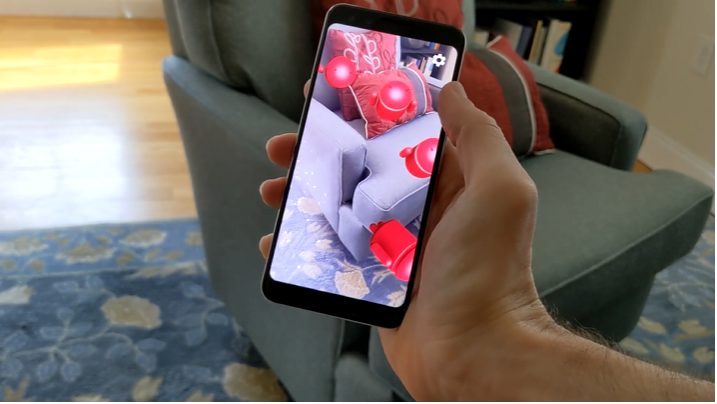
\includegraphics[width=0.8\textwidth]{../../resources/images/OrientedPoints/points1.png}}%
				{Fonte: \url{https://developers.google.com/ar/develop/java/depth/developer-guide}}
				\caption{Esempio di punti orientati su una superficie arbitraria}
				\label{fig: surf-arb}
		\end{figure}
		
		
\end{document}